<<<<<<< HEAD
%LTeX: language=it
\subsection{UC 7 - Modifica di un oggetto} \label{sec:UC7}
    \begin{figure}[h]
        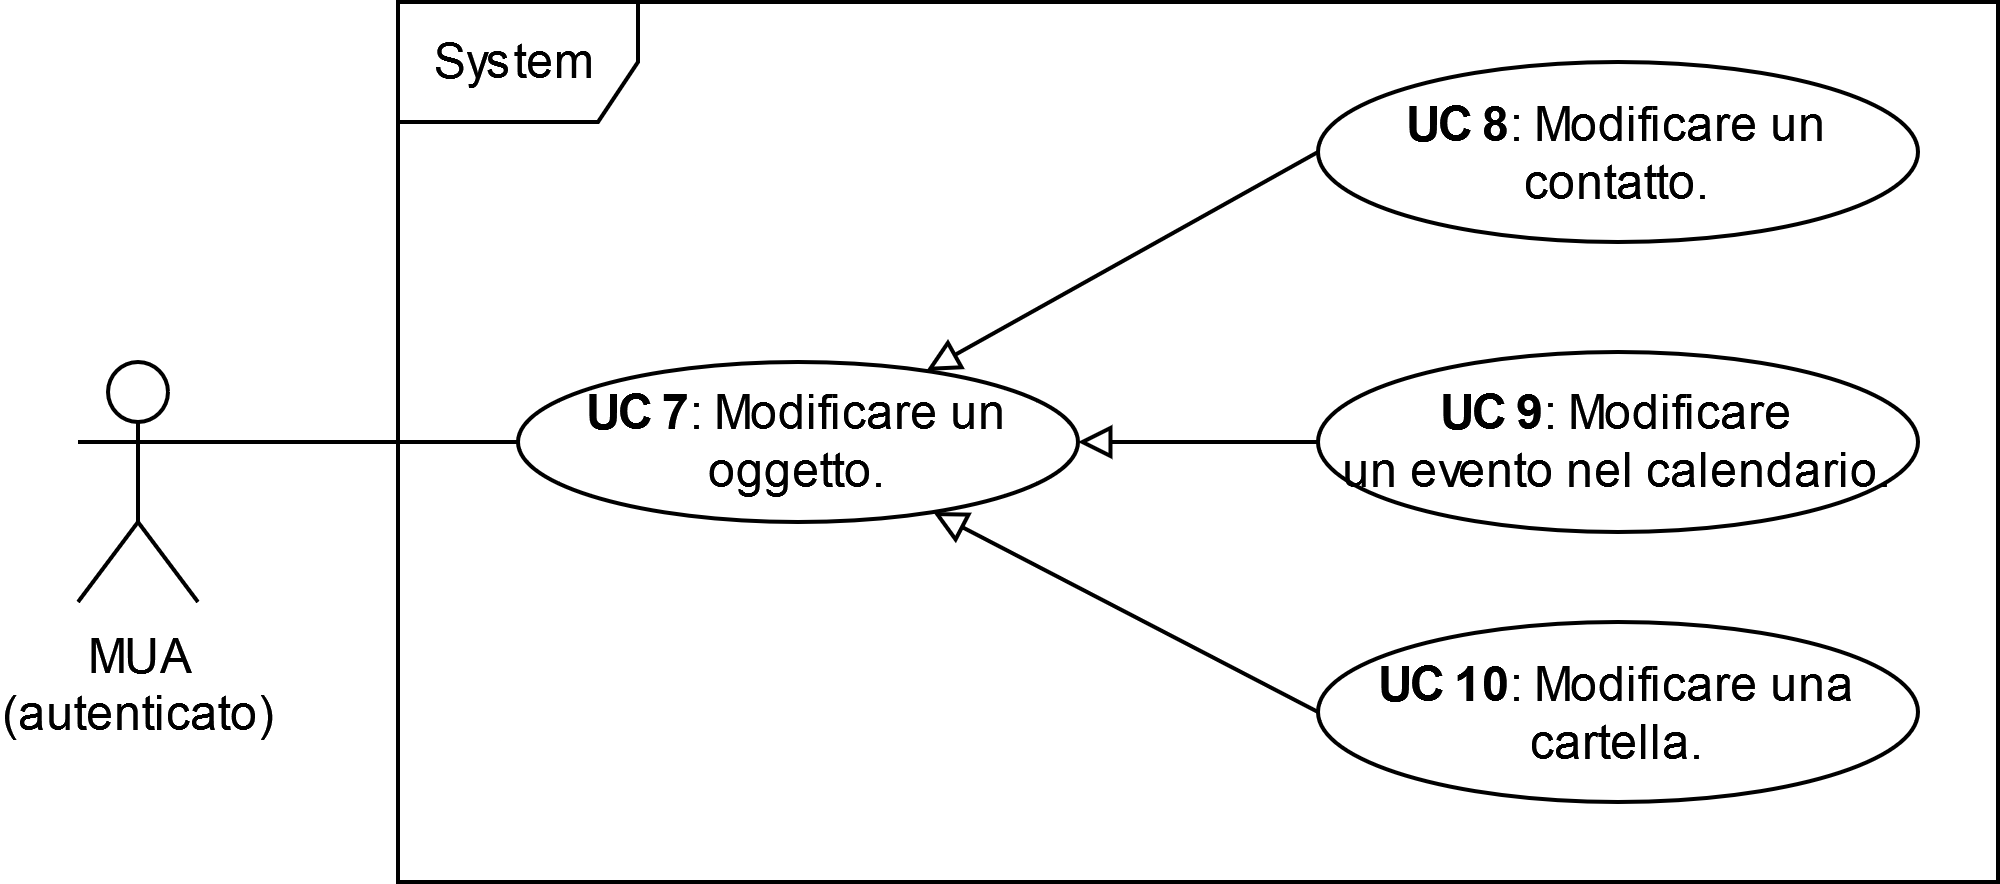
\includegraphics[width=0.85\textwidth]{sections/uc_imgs/UC07.png}
        \centering
        \caption{Diagramma UC 7.}
    \end{figure}
    \begin{itemize}
        \item \textbf{Attore principale}: MUA;
        \item \textbf{Descrizione}: il MUA deve poter modificare un oggetto nel sistema;
        \item \textbf{Precondizioni}: l’account che il MUA gestisce è registrato nel sistema, e ha un connessione aperta con il sistema ed è autenticato;
        \item \textbf{Postcondizioni}: il MUA modifica un oggetto, il suo nuovo stato viene salvato nel sistema;
        \item \textbf{Scenario principale}:
            \begin{enumerate}
                \item il MUA invia le informazioni per aggiornare l'oggetto nel sistema;
                \item il sistema salva il nuovo stato dell'oggetto;
            \end{enumerate}
        \item \textbf{Inclusioni}: nessuna;
        \item \textbf{Generalizzazioni}:
            \begin{itemize}
                \item il MUA modifica un contatto (\hyperref[sec:UC8]{UC 8});
                \item il MUA modifica un evento nel calendario (\hyperref[sec:UC9]{UC 9});
                \item il MUA modifica una cartella (\hyperref[sec:UC10]{UC 10});
            \end{itemize}
        \item \textbf{Estensioni}: nessuna.
    \end{itemize}
=======
\subsection{UC 7 - Creazione condivisione cartella} \label{sec:UC7}

    \begin{itemize}
        \item \textbf{Attore principale}: MUA;
        \item \textbf{Descrizione}: il MUA deve poter creare una condivisione di una cartella nel sistema;
        \item \textbf{Precondizioni}: il MUA sta usando la funzionalità di creazione di una condivisione;
        \item \textbf{Postcondizioni}: il sistema condivide la cartella con l'indirizzo e-mail fornito dal MUA;
        \item \textbf{Scenario principale}:
            \begin{enumerate}
                \item il MUA trasmette l'id della cartella da condividere (\hyperref[sec:UC7.1]{UC 7.1});
                \item il MUA trasmette l'indirizzo e-mail a cui condividere (\hyperref[sec:UC7.2]{UC 7.2});
                \item il sistema condivide la cartella;
            \end{enumerate}
        \item \textbf{Inclusioni}: nessuna;
        \item \textbf{Generalizzazioni}: nessuna;
        \item \textbf{Estensioni}: nessuna.
    \end{itemize}

    \begin{figure}[H]
        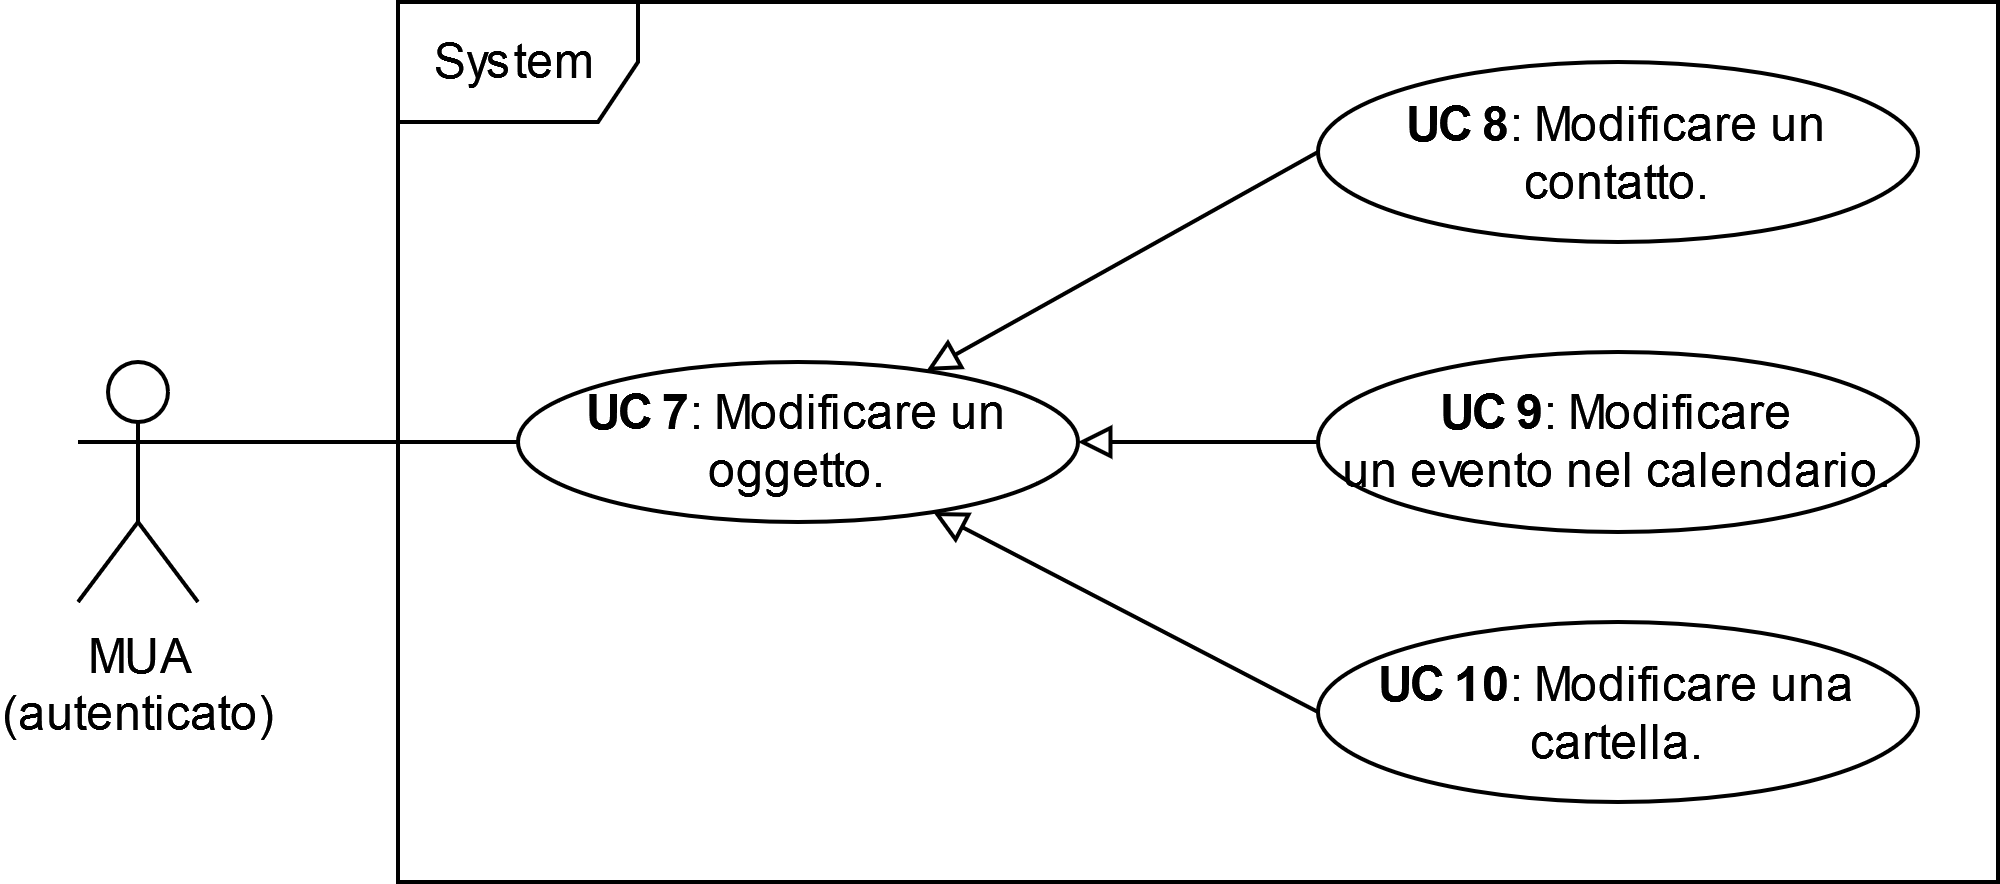
\includegraphics[width=0.85\textwidth]{sections/uc_imgs/UC07.png}
        \centering
        \caption{Diagramma sotto-casi UC 7}
    \end{figure}

    \subsubsection{UC 7.1 - Trasmette id cartella} \label{sec:UC7.1}
    \begin{itemize}
        \item \textbf{Attore principale}: MUA;
        \item \textbf{Descrizione}: il MUA trasmette l'id della cartella per condividere la cartella;
        \item \textbf{Precondizioni}: il MUA sta usando la funzionalità di creazione condivisione di una cartella;
        \item \textbf{Postcondizioni}: il sistema conosce l'id della cartella da condividere;
        \item \textbf{Scenario principale}:
            \begin{enumerate}
                \item il MUA invia l'id della cartella per condividere la cartella;
            \end{enumerate}
        \item \textbf{Inclusioni}: nessuna;
        \item \textbf{Generalizzazioni}: nessuna;
        \item \textbf{Estensioni}:
            \begin{enumerate}[label=\alph*.]
                \item il sistema non riesce a condividere la cartella perché l'id della cartella fornito non è stato trovato:
                \begin{enumerate}[label=\arabic*.]
                    \item il sistema ritorna un errore al MUA di cartella non trovata (\hyperref[sec:UC7.3]{UC 7.3}).
                \end{enumerate}
            \end{enumerate}
    \end{itemize}


    \subsubsection{UC 7.2 - Trasmette indirizzo contatto} \label{sec:UC7.2}
    \begin{itemize}
        \item \textbf{Attore principale}: MUA;
        \item \textbf{Descrizione}: il MUA trasmette l'indirizzo e-mail per la condivisione al sistema;
        \item \textbf{Precondizioni}: il MUA sta usando la funzionalità di creazione condivisione di una cartella;
        \item \textbf{Postcondizioni}: il sistema conosce l'indirizzo e-mail a cui condividere;
        \item \textbf{Scenario principale}:
            \begin{enumerate}
                \item il MUA invia l'indirizzo e-mail per la condivisione al sistema;
                \item il sistema controlla che le informazioni ricevute rispettino il seguente requisito minimo:
                    \begin{itemize}
                        \item l'indirizzo e-mail del contatto non è una stringa vuota;
                    \end{itemize}
            \end{enumerate}
        \item \textbf{Inclusioni}: nessuna;
        \item \textbf{Generalizzazioni}: nessuna;
        \item \textbf{Estensioni}:
            \begin{enumerate}[label=\alph*.]
                \item il sistema non riesce a creare la condivisione della cartella perché l'indirizzo e-mail fornito non è valido:
                \begin{enumerate}[label=\arabic*.]
                    \item il sistema ritorna un errore al MUA di indirizzo e-mail non valido (\hyperref[sec:UC7.4]{UC 7.4}).
                \end{enumerate}
            \end{enumerate}
    \end{itemize}


\subsubsection{UC 7.3 - Ritorna errore cartella non trovata} \label{sec:UC7.3}
    \begin{itemize}
        \item \textbf{Attore principale}: MUA;
        \item \textbf{Descrizione}: il sistema non riesce a condividere la cartella perché la cartella non è stata trovata;
        \item \textbf{Precondizioni}: il MUA ha inviato l'id della cartella da condividere;
        \item \textbf{Postcondizioni}: il sistema non condivide la cartella, il MUA è stato notificato dell'errore;
        \item \textbf{Scenario principale}:
            \begin{enumerate}
                \item il sistema non trova la cartella con l'identificativo fornito dal MUA;
                \item il sistema non condivide la cartella e notifica il MUA dell'errore;
            \end{enumerate}
        \item \textbf{Inclusioni}: nessuna;
        \item \textbf{Generalizzazioni}: nessuna;
        \item \textbf{Estensioni}: nessuna.
    \end{itemize}

    \subsubsection{UC 7.4 - Ritorna errore indirizzo e-mail non valido} \label{sec:UC7.4}
    \begin{itemize}
        \item \textbf{Attore principale}: MUA;
        \item \textbf{Descrizione}: il sistema non riesce a condividere la cartella perché l'indirizzo e-mail del contatto non rispetta i requisiti;
        \item \textbf{Precondizioni}: il MUA ha inviato l'indirizzo e-mail a cui condividere;
        \item \textbf{Postcondizioni}: il sistema non condivide la cartella, il MUA è stato notificato dell'errore;
        \item \textbf{Scenario principale}:
            \begin{enumerate}
                \item il sistema controlla la sintassi dell'indirizzo e-mail e trova un errore;
                \item il sistema non condivide la cartella e notifica il MUA dell'errore;
            \end{enumerate}
        \item \textbf{Inclusioni}: nessuna;
        \item \textbf{Generalizzazioni}: nessuna;
        \item \textbf{Estensioni}: nessuna.
    \end{itemize}
>>>>>>> 177cc19041165c8485927b56b5ea094ec2cbcfb6
